\section{Protocol-Dependent Geometric Signatures}
\label{sec:phenomenon}

\subsection{Controlled diagnostic setting}
\label{sec:phenomenon-setting}

We retrospectively compare four matched-width \textsc{Qwen2.5}-derived 1.5B variants
\citep{qwen25-2024,qwen25-math-2024,deepseek-r1-2025}.  They share width,
tokenizer, prompt, decoding rule, and diagnostic problem slice, but they are not
a strict sequence of immediate checkpoints.  Consequently, the comparison asks
whether the checkpoints exhibit different trajectory--correctness associations
under one fixed protocol; it does not identify a unique causal contribution of
any individual post-training operation.
We use SFT for supervised fine-tuning, DPO for direct preference optimization,
and CPT for continued pretraining in Table~\ref{tab:model-lineage}.

\begin{table}[tbp]
\centering
\scriptsize
\setlength{\tabcolsep}{1.5pt}
\caption{Controlled diagnostic family.  Accuracies from the shared retrospective
512-token extraction protocol describe the available correct/incorrect mix;
they are not official benchmark results and are unrelated to the corrected
steering baseline in Section~\ref{sec:crosssteer}.}
\label{tab:model-lineage}
\resizebox{\columnwidth}{!}{%
\begin{tabular}{@{}lllr@{}}
\toprule
Variant & Exact checkpoint & Post-training contrast & Acc. \\
\midrule
\textsc{Base} & Qwen2.5-1.5B & pretraining & 0.37 \\
\textsc{Instruct} & Qwen2.5-1.5B-Instruct & general SFT + DPO & 0.60 \\
\textsc{Math-Instruct} & Qwen2.5-Math-1.5B-Instruct & math CPT/SFT & 0.78 \\
\textsc{R1-Distill} & DeepSeek-R1-Distill-Qwen-1.5B & R1-trace distillation & 0.32 \\
\bottomrule
\end{tabular}%
}
\end{table}

For each model, we extract trajectories on the same 100 GSM8K test problems
(GSM8K IDs 0--99)
\citep{cobbe-etal-2021-training}.  These IDs also form the source-direction
training split in Section~\ref{sec:crosssteer}; the signatures never select a
steering layer, sign, or strength, and steering evaluation uses the disjoint
IDs 100--299.  We compute the seven functionals from
Section~\ref{sec:framework} at all 29 layers, residualize log generated length, and
form one signature matrix $S_i\in[0,1]^{7\times29}$ per checkpoint
(Figure~\ref{fig:phen-heatmap}).

\begin{figure*}[tbp]
\centering
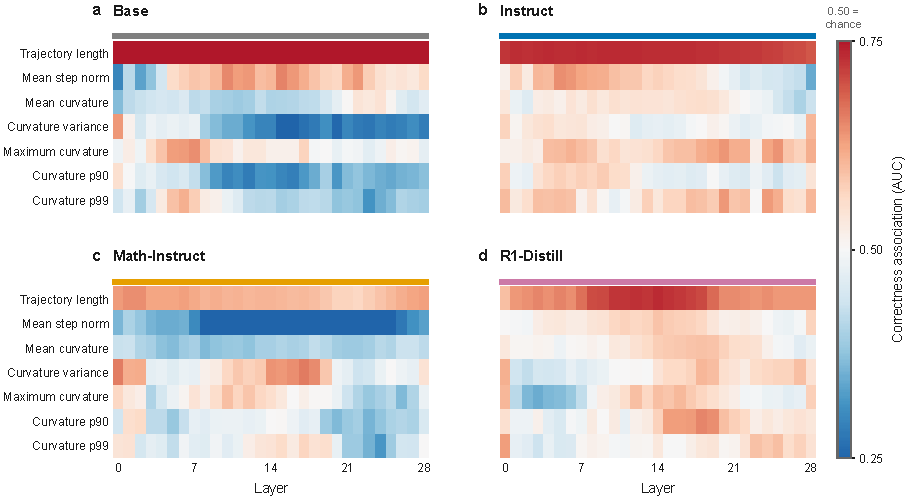
\includegraphics[width=0.98\linewidth]{figures/fig2_signature_heatmaps.pdf}
\caption{Length-residualized metric--layer AUCs for four matched checkpoints;
the shared scale is centered at chance (0.50); the axis label \emph{Mean step
norm} denotes \textsc{StepNorm}.  These are descriptive
associations, not a mechanism, taxonomy, or steering rule.}
\label{fig:phen-heatmap}
\end{figure*}

\subsection{Descriptive distance and its stability boundary}

Table~\ref{tab:phen-distance} gives pairwise distances between centered signature
matrices at the original 512-token budget and a retrospective 2048-token sensitivity comparison;
Figure~\ref{fig:phen-distance-stability} visualizes the paired changes.
The distances are nonzero in both settings, indicating that the checkpoint summaries
differ under each fixed extraction protocol.  The 2048-token artifacts are legacy
retrospective data that do not preserve the full decoder and replay provenance
required by our revision protocol, so this comparison is descriptive and not a
fresh confirmation result.  Their magnitudes change with the
generation budget, and the identity of the largest-distance pair changes, whereas
the closest pair remains \textsc{Instruct}--\textsc{R1-Distill}.  We therefore treat
the distance matrix as a protocol-specific descriptive summary rather than a
protocol-invariant post-training fingerprint.

\begin{table}[tbp]
\centering
\footnotesize
\setlength{\tabcolsep}{5.5pt}
\caption{Pairwise signature distance on the diagnostic GSM8K slice,
$d(S_i,S_j)=\lVert(S_i-0.5)-(S_j-0.5)\rVert_F$.  The 2048-token block is a
retrospective sensitivity comparison using legacy artifacts, not a fresh
confirmation; the closest pair persists while the largest pair changes.}
\label{tab:phen-distance}
\textit{512-token diagnostic}\\[3pt]
\begin{tabular}{@{}lcccc@{}}
\toprule
& \textsc{Base} & \textsc{Inst.} & \textsc{Math} & \textsc{R1} \\
\midrule
\textsc{Base} & 0.00 & 1.83 & 2.63 & 2.13 \\
\textsc{Inst.} & 1.83 & 0.00 & 2.18 & 1.13 \\
\textsc{Math} & 2.63 & 2.18 & 0.00 & 2.09 \\
\textsc{R1} & 2.13 & 1.13 & 2.09 & 0.00 \\
\bottomrule
\end{tabular}\\[7pt]
\textit{2048-token retrospective}\\[3pt]
\begin{tabular}{@{}lcccc@{}}
\toprule
& \textsc{Base} & \textsc{Inst.} & \textsc{Math} & \textsc{R1} \\
\midrule
\textsc{Base} & 0.00 & 1.81 & 2.27 & 2.44 \\
\textsc{Inst.} & 1.81 & 0.00 & 2.06 & 1.54 \\
\textsc{Math} & 2.27 & 2.06 & 0.00 & 1.57 \\
\textsc{R1} & 2.44 & 1.54 & 1.57 & 0.00 \\
\bottomrule
\end{tabular}
\end{table}

\begin{figure*}[tbp]
\centering
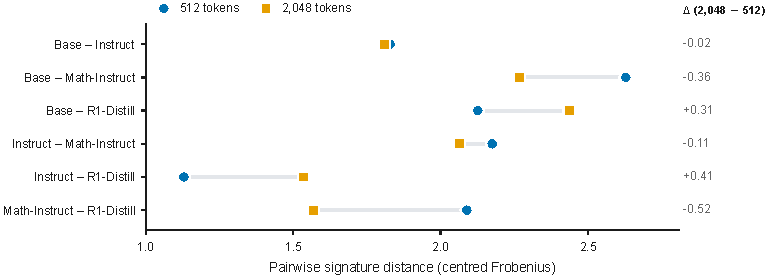
\includegraphics[width=0.88\linewidth]{figures/fig_signature_distance_stability.pdf}
\caption{Pairwise signature distances at 512 and 2,048 tokens; connectors
show within-pair budget change.  This is a descriptive stability audit, not a
model or intervention-selection rule.}
\label{fig:phen-distance-stability}
\end{figure*}

\paragraph{Bootstrap stability audit.}
To quantify the uncertainty behind the displayed nearest-neighbor relations, we
resample shared problem IDs 1,000 times and recompute the directed nearest
neighbor from the matched signature cells.  At 1.5B, Base selects Instruct in
0.631 of resamples, Instruct selects Base in 0.695, and Math selects R1-Distill
in 0.689; the R1-Distill relation is diffuse (Base 0.460, Instruct 0.379).  In
the retrospective 7B audit, Base--R1 and R1--Base are stable (0.993 and 0.995),
whereas Instruct--Base and Math--Base are not (0.506 and 0.512).
These changes have several plausible statistical sources: changing the generation
budget changes stopping and path sampling, changing the slice changes the finite
AUC estimates, and changing scale changes the hidden representation itself.  The
available audits distinguish these sensitivities but do not identify one unique
cause.  We therefore report topology as a stability diagnostic, not as a
post-training explanation.  A separately preregistered fresh confirmation
chain (Qwen 512/2048 and Gemma 512/2048 cells) did not enter confirmatory
analysis because at least one required model in each cell exceeded the
predeclared 25\% truncation ceiling; the signature matrices here are
therefore retained as retrospective, protocol-bounded descriptive evidence,
and the non-qualification is reported rather than treated as evidence about
geometry.  The 25\% ceiling is specific to this confirmatory chain; the
512-token OOD stress envelope in Section~\ref{sec:crosssteer} has a separate
4,096-token low-truncation companion.  The retrospective 7B distance matrix behind the
7B bootstrap numbers is in Appendix~\ref{app:scale-7b} (Table~\ref{tab:scale7b-distance}).

\paragraph{What this supports.}
At 512 tokens, \textsc{Base}--\textsc{Math-Instruct} is the largest displayed
pairwise distance and \textsc{Instruct}--\textsc{R1-Distill} the smallest; at
2048 tokens the smallest pair persists but the largest becomes
\textsc{Base}--\textsc{R1-Distill}.  We therefore
claim only that the matched checkpoints have different metric--layer
correctness-association summaries under the specified protocol.  We do not claim
a stable cluster structure, a universal model fingerprint, or that the distance isolates one
post-training algorithm from all lineage differences.

\paragraph{Localized signals are descriptive hypotheses.}
The heatmaps include localized StepNorm and CurvMean associations, including a
curvature orientation that differs for \textsc{R1-Distill} in this slice.  Such
patterns identify candidate descriptive differences, but they are not used to
choose a target, layer, sign, or strength for an intervention.  The controlled
GeoVote audit in Section~\ref{sec:geovote} and the frozen steering comparison in
Section~\ref{sec:crosssteer} test whether any of these associations provide
utility beyond output-level and activation-steering controls.

\paragraph{Correctness-direction visualization.}
Figure~\ref{fig:phen-separation} projects states onto a direction estimated from
correct and incorrect trajectories in the same model.  It is included solely as
an intuitive visualization of a high-dimensional label-conditioned separation;
it is neither an out-of-sample verifier nor evidence that the corresponding
direction is a causal reasoning mechanism.

\begin{figure*}[tbp]
\centering
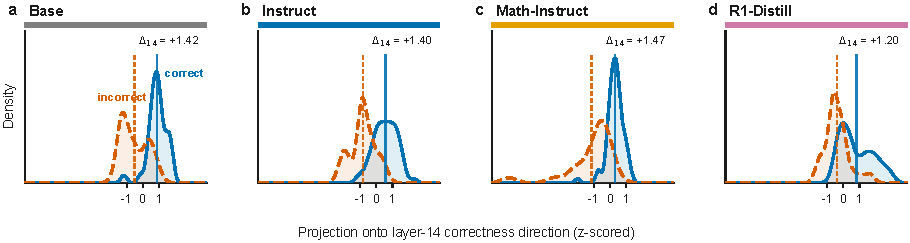
\includegraphics[width=0.98\linewidth]{figures/fig3_correctness_separation.pdf}
\caption{Correct and incorrect generations projected onto each model's
layer-14 correctness direction.  Means are shown after display normalization;
direction and labels come from the same diagnostic split, so the view is
descriptive.}
\label{fig:phen-separation}
\end{figure*}
